\chapter[Muscle Force Generation: The Biological Engine]{Muscle Force Generation:\\The Biological Engine}
\label{ch:muscle-force-generation}
\raggedbottom
\index{wrist torque}
\index{slow-twitch}
\index{shoulder torque}
\index{series elastic element}
\index{sequencing}
\index{sarcomere overlap}
\index{sarcomere}
\index{pre-activation}
\index{physiological cross-sectional area}
\index{pennation angle}
\index{peak torques}
\index{parallel elastic element}
\index{neural command}
\index{neural activation}
\index{muscle architecture}
\index{force-velocity curve}
\index{force-length curve}
\index{fiber types}
\index{fast-twitch}
\index{excitation-contraction coupling}
\index{elbow torque}
\index{eccentric contraction}
\index{drift field}
\index{control field}
\index{control affine}
\index{contractile element}
\index{concentric contraction}
\index{activation time constant}
\index{actin-myosin}
\index{PCSA}
\index{Hill's equation}
\index{Hill muscle model}

\begin{laymansbox}{Why Muscle Biology Matters for Your Swing}{context:muscle-matters}
The nervous system prepares muscle activity; muscles pull on tendons; tendon forces act through changing moment arms; the coupled body and club respond. Each link matters. A fast clubhead does not tell us how fast a particular muscle fiber is shortening. A small net joint torque does not tell us that the surrounding muscles are relaxed. Understanding these distinctions lets us ask a useful golf question: which changes in preparation or ongoing activation can still change the impact conditions, by how much, and with what consequences elsewhere in the body?
\end{laymansbox}

This chapter develops a reproducible teaching model before discussing measurements and training. Its numerical examples are manufactured calculations, not estimates of a particular golfer. The purpose is to connect biological limitations to mechanics without turning a plausible mechanism into an unsupported claim that every player must use one sequence. The model omits fatigue, injury, detailed neural circuitry and many tissue effects; those omissions define the questions it can answer.

\section{Muscle Architecture: What a Muscle Actually Is}

\begin{definition}{The Muscle Hierarchy}{muscle-hierarchy}
A skeletal muscle contains fascicles, which contain muscle fibers. Each fiber is a cell containing myofibrils with sarcomeres arranged along their length. Actin and myosin interact within these repeating units. Sarcomeres in series contribute length and shortening excursion; contractile structures in parallel contribute force. A muscle can produce active tension while shortening, holding approximately constant length or being lengthened by its load. The word contraction does not require visible shortening.
\end{definition}

An electrical signal initiates processes that raise calcium availability within the fiber. Cross-bridge cycling couples chemical energy to force and motion. ATP binding allows myosin to detach from actin, hydrolysis prepares another cycle, and calcium handling also consumes energy. This mechanism is different from stretching a passive rubber band. The band can return energy previously stored in it; an activated muscle can convert chemical energy into mechanical work. A loaded muscle also contains passive structures, so measured total tension need not disappear when neural excitation stops. \citep{OpenStax2022Contraction}

\begin{principle}{Muscle Fiber Types and Their Roles}{principle:fiber-types}
Fiber classifications summarize differences in contractile speed and metabolic properties. Slow oxidative fibers tend to resist fatigue; fast oxidative and fast glycolytic categories describe different combinations of speed and energy supply. These categories do not give a universal percentage composition for every muscle or golfer. Nor does a fast clubhead establish the player's fiber composition. Fiber size, recruitment, architecture, training history and task coordination are separate quantities. \citep{OpenStax2022FiberTypes}
\end{principle}

\begin{definition}{Muscle Architectural Parameters}{muscle-architecture}
Let $\ell^M$ be fiber length in meters, $\ell^M_{\mathrm{opt}}$ its reference optimal length, and $\alpha$ the angle between fibers and the tendon line. For approximately parallel, equal-length fibers at the reference configuration, a volume-based physiological cross-sectional area is
\[
A_{\mathrm{PCSA}}=\frac{V_M}{\ell^M_{\mathrm{opt}}}
=\frac{m_M}{\rho_M\ell^M_{\mathrm{opt}}},
\qquad F_0=\sigma_0 A_{\mathrm{PCSA}}.
\]
Here $m_M$ is muscle mass, $\rho_M$ density, and $\sigma_0$ specific tension in compatible units. We define $F_0$ along the fiber direction. Its tendon-direction projection at the reference pennation is $F_0\cos\alpha_0$. Some sources incorporate this projection in their area or maximum-force convention; applying it again would double-count pennation. These reference parameters are not recalculated by substituting the instantaneous fiber length into the area formula.
\end{definition}

For an explicitly hypothetical area of $3\,\mathrm{cm^2}$ and specific tension of $30\,\mathrm{N/cm^2}$, $F_0=90\,\mathrm{N}$. At $\alpha_0=20^\circ$ its projection is about $84.6\,\mathrm{N}$. This arithmetic is transparent; interpreting either input as a measured value for a named golf muscle would require anatomical evidence. Increasing fiber length at fixed muscle volume trades parallel area for excursion capacity in this simplified architecture. Increasing pennation changes both packing and projection, so the cosine alone does not establish whether one architecture is stronger.

The source of anatomical parameters matters. Holzbaur and colleagues' upper-extremity model includes shoulder-to-finger geometry and comparisons with moment arms and isometric moment capacity. Its tendon slack lengths were selected using additional constraints, and the authors identify sensitivity and shoulder-geometry limitations. It is a starting model, not validation of muscle force during a golf swing. \citep{Holzbaur2005} Rajagopal and colleagues' gait model instead uses muscle-tendon actuators in the lower limbs and ideal torque actuators for the upper body. It cannot supply evidence for detailed forearm muscle parameters merely because its title says full-body. \citep{Rajagopal2016}

\section{The Force-Length Relationship}

\begin{laymansbox}{Strength Changes With Joint Angle}{context:force-length-intuition}
Changing joint angle changes muscle paths, fiber lengths and moment arms. Active force depends in part on filament interaction, while passive tension increases as passive structures are loaded. Joint strength therefore need not peak at the angle where one muscle's active fiber force peaks. Antagonists, other muscles crossing the joint and the test apparatus also contribute to the measured moment.
\end{laymansbox}

Normalize fiber length as $\lambda=\ell^M/\ell^M_{\mathrm{opt}}$. A convenient illustrative active curve is
\begin{equation}
f_L(\lambda)=\exp\!\left[-\left(\frac{\lambda-1}{\gamma}\right)^2\right],
\qquad \gamma=0.5.
\label{eq:active-force-length}
\end{equation}
This Gaussian has a maximum of one at $\lambda=1$. It has neither an exactly flat plateau nor a finite length at which it becomes exactly zero. At $\lambda=0.8$ and $1.2$, it gives $e^{-0.16}\approx0.8521$; at $0.5$ and $1.5$, it still gives $e^{-1}\approx0.3679$. Thus it should not be extrapolated as a literal prediction of filament overlap at extreme lengths. The parameter $\gamma$ is a declared teaching choice, not a universal tissue measurement.

\begin{principle}{Regions of the Force-Length Curve}{principle:fl-regions}
Distinguish the active-force curve from total force. Activation can scale active force while passive structures contribute separately. A low active-force multiplier at short length is not the same mechanism as low neural recruitment. At longer lengths, decreasing active force can coexist with increasing passive tension. A model should state both contributions and the lengths over which its fitted curves are supported.
\end{principle}

For a nonnegative passive teaching curve, choose $k_P=4$ and $\epsilon_P=0.6$:
\begin{equation}
f_P(\lambda)=
\begin{cases}
0,&\lambda\leq1,\\
\dfrac{e^{k_P(\lambda-1)}-1}{e^{k_P\epsilon_P}-1},&\lambda>1.
\end{cases}
\label{eq:passive-force-length}
\end{equation}
The threshold, shape and normalization are explicit: $f_P(1)=0$ and $f_P(1.6)=1$. At $1.2$ it is about $0.12227$. The expression never generates passive compression below its slack threshold. Its right derivative at the threshold differs from the left derivative; a differentiable simulation model would require an appropriate transition if a solver or sensitivity calculation needs one.

With dimensionless activation $a\in[0,1]$ and the velocity multiplier defined next, total fiber-direction force is
\begin{equation}
F_M=F_0\{a f_L(\lambda)f_V(w)+f_P(\lambda)\}.
\label{eq:total-muscle-force}
\end{equation}
This expression deliberately omits viscous damping and history effects. It distinguishes the active component from passive tension but does not resolve every structure inside a real muscle.

\begin{example}{Latissimus Dorsi Through the Swing}{lat-force-length}
A statement that the latissimus is near its optimal length at a particular swing phase requires more than an image of the pose. The shoulder girdle configuration, muscle path, tendon extension, pennation and reference fiber length all affect the inference. Suppose a model gives $\lambda=1.2$ and $a=0.7$ at zero fiber velocity. Our chosen curves give
\[
F_M/F_0\approx0.7(0.8521)+0.12227=0.7188.
\]
 That is a calculation conditional on model inputs; it does not establish either input for a golfer. Testing the claim requires checking the modeled geometry and measured motion, and reporting sensitivity to uncertain parameters.
\end{example}

\section{The Force-Velocity Relationship: Hill's Equation}

\begin{laymansbox}{The Central Constraint: Force Depends on Fiber Speed}{context:force-velocity-intuition}
A muscle fiber shortening rapidly generally has less active force capacity than the same fiber shortening slowly under comparable conditions. This statement concerns local fiber velocity. A muscle can move quickly through the room while its fiber length barely changes, and a moving tendon can stretch while the fibers shorten. Clubhead speed alone identifies neither motion.
\end{laymansbox}

Choose the shortening-positive convention
\[
w=-\frac{\dot\ell^M}{V_{\max}},
\qquad V_{\max}=\nu\ell^M_{\mathrm{opt}},
\]
where $\dot\ell^M$ is positive for lengthening, $V_{\max}$ is in $\mathrm{m/s}$, and $\nu$ is in fiber lengths per second. For example, $2$--$4$ lengths/second for a $0.10\,\mathrm{m}$ reference fiber means $0.2$--$0.4\,\mathrm{m/s}$. Confusing these units produces order-of-magnitude errors.

A normalized concentric Hill-type relation is
\begin{equation}
f_V(w)=\frac{1-w}{1+w/k},
\qquad 0\leq w\leq1,\quad k=0.4.
\label{eq:hill-concentric}
\end{equation}
It is hyperbolic, not linear. It equals one at zero shortening velocity and zero at the declared unloaded shortening limit. Extrapolating it above $w=1$ would produce negative active force; that extrapolation is outside this teaching law's domain. A simulation encountering that condition needs a stated treatment and a check that the assumed force equilibrium is physically and numerically admissible.

\begin{principle}{Concentric vs. Eccentric: The Asymmetry}{principle:ecc-vs-conc}
For lengthening, use the following explicitly constructed illustration:
\[
f_V(w)=1+(F_\infty-1)\frac{-w}{c-w},\qquad w\leq0,
\]
with $F_\infty=1.4$. Choose $c=4/35$ so that $c(1+1/k)=F_\infty-1$. It approaches $1.4$ as $w\to-\infty$, equals one at zero and has the same derivative there as the concentric branch. These choices make the joined velocity curve continuously differentiable at zero. They are not the published Thelen equation and do not establish a universal eccentric-force ceiling. Particular muscle models use different fitted curves, constraints and numerical regularizations. \citep{millard2013flexing}
\end{principle}

Active shortening power is $P_{\mathrm{CE}}=-F_{\mathrm{CE}}\dot\ell^M$. At full activation and optimal length, normalized power is
\[
P_{\mathrm{CE}}/(F_0V_{\max})=w f_V(w).
\]
 Differentiating gives the interior maximum
\[
w_* = \sqrt{k^2+k}-k\approx0.34833,
\qquad \frac{P_*}{F_0V_{\max}}\approx0.12133.
\]
Maximum force and maximum shortening power occur at different speeds. Isometric force can be substantial while fiber shortening power is zero. During active lengthening, this sign convention gives negative mechanical power: the contractile component absorbs mechanical energy while still requiring metabolic processes.

\begin{figure}[H]
\centering
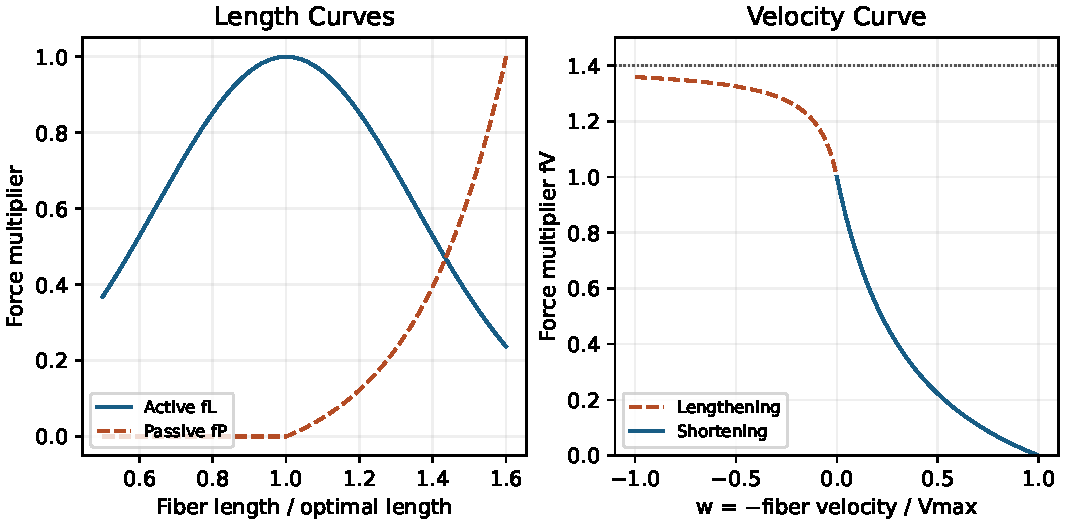
\includegraphics[width=\linewidth]{figures/muscle_force_curves.pdf}
\caption{Declared Teaching Curves: Active and Passive Length Multipliers, and the Joined Velocity Law. The Parameters Are Illustrative, Not Golfer Measurements.}
\label{fig:muscle-force-curves}
\end{figure}

\begin{principle}{What High Club Speed Does and Does Not Establish}{drift:muscle-fv}
High club speed changes the mechanical problem, but it does not insert that speed directly into $f_V$. First obtain each muscle-tendon path velocity from joint motion, then separate tendon and fiber motion. Likewise, $mv^2$ has units of energy, not force; a centripetal force estimate needs a radius, $mv^2/R$, and a specified trajectory. Gravitational force near Earth's surface does not grow with swing speed. Configuration-dependent inertial and velocity-coupling effects require the equations of motion, not a comparison of unlike speed scales.
\end{principle}

\begin{example}{Numerical Estimate: Local Wrist Muscle Force}{wrist-fv}
Consider a hypothetical unpennated muscle with a rigid tendon, constant moment arm $r=0.02\,\mathrm{m}$, reference fiber length $0.10\,\mathrm{m}$ and $\nu=10\,\mathrm{s^{-1}}$. If the relevant joint alone rotates at $8.75\,\mathrm{rad/s}$ in the shortening direction, $-\dot\ell^M=r\dot q$, giving $0.175\,\mathrm{m/s}$ and $V_{\max}=1\,\mathrm{m/s}$. Therefore $w=0.175$ and
\[
f_V=0.825/1.4375\approx0.5739.
\]
 With $F_0=100\,\mathrm{N}$, $a=1$, $\lambda=1$ and no passive force, the tendon force is $57.39\,\mathrm{N}$ and moment $1.148\,\mathrm{N\,m}$. These inputs do not describe measured extensor carpi radialis brevis (ECRB) force at impact. Dividing clubhead speed by a guessed lever length cannot replace the required joint and path kinematics.
\end{example}

\section{Muscle Activation Dynamics}

\begin{laymansbox}{Why Muscles Are Slow to Respond}{context:activation-delay-intuition}
Neural excitation $u$ is an input to the muscle model. Activation $a$ describes its evolving active state; it is not identical to the command or to measured electromyography (EMG) amplitude. Tendon force follows from activation together with length, velocity and elastic loading. Consequently, a command change, an EMG onset and an external force onset are different events.
\end{laymansbox}

For an elementary model, choose a fixed time constant $\tau_a>0$:
\begin{equation}
\dot a=\frac{u-a}{\tau_a},\qquad 0\leq u,a\leq1.
\label{eq:activation-rise}
\end{equation}
For a constant command starting at $t=0$, direct integration gives
\begin{equation}
a(t)=u+(a_0-u)e^{-t/\tau_a}.
\label{eq:activation-fall}
\end{equation}
The same equation describes decay when $u<a_0$. This fixed-constant model is intentionally simpler than activation-dependent rise and fall laws. Published implementations differ; the chosen law and any minimum activation must be specified before comparing simulations. \citep{OpenSimActivationDynamics}

For $a_0=0$, $u=1$ and $\tau_a=25\,\mathrm{ms}$, activation reaches $63.2\%$ after one time constant, $50\%$ after $17.33\,\mathrm{ms}$ and $95\%$ after $74.89\,\mathrm{ms}$. At $50\,\mathrm{ms}$ it is about $0.8647$. Exact equality to one occurs only asymptotically. A time constant therefore is not a period of complete inactivity followed by full force. Nor does $95\%$ activation imply $95\%$ of isometric joint torque during a moving, compliant task.

A numerical solver adds another issue. Forward Euler with a $5\,\mathrm{ms}$ step gives $a_n=1-0.8^n$, reaching $95\%$ at step 14, or $70\,\mathrm{ms}$. The exact continuous solution crosses that threshold at $74.89\,\mathrm{ms}$. Refining the time step or using a suitable integrator reduces this numerical discrepancy. It is not evidence for a faster physiological response.

\begin{definition}{Electromechanical Delay}{emd}
An experimentally reported delay depends on the selected start and end events, detection thresholds, contraction protocol and loading. Nordez and colleagues used ultrasound during electrically evoked gastrocnemius contractions to distinguish aspects of fascicle and tendon onset. That experiment does not supply a universal visual-reaction delay or golf-wrist latency. \citep{Nordez2009Delay} Adding an EMG-to-force delay to an activation time constant can double-count processes if both quantities already describe overlapping parts of the response. A pure delay may be added to a model, but its location and measurement basis must be explicit.
\end{definition}

\begin{example}{Reaction Time in the Golf Downswing}{reaction-time}
Suppose a command changes $70\,\mathrm{ms}$ before impact and a separately specified pure transmission delay is $20\,\mathrm{ms}$. Our activation model then has $50\,\mathrm{ms}$ to respond. Its activation increment from zero is $0.8647$ at impact. If the same command had already established activation earlier, the starting state would be different. Conversely, a sensory correction requiring additional detection and processing could leave less time. This timing ledger is a conditional example, not a measured sequence of events in every downswing. Preparation and a new response must be compared from their actual initial states.
\end{example}

\section{The Hill-Type Muscle Model}

\begin{definition}{Hill-Type Muscle Model Components}{hill-model}
The contractile element (CE) and passive parallel element (PEE) act along the fiber direction. Their combined force is projected through pennation onto the series tendon, also called the series elastic element (SEE). With a massless connection and no extra damper in this teaching model,
\begin{equation}
F_T=(F_{\mathrm{CE}}+F_{\mathrm{PE}})\cos\alpha=F_M\cos\alpha.
\label{eq:total-hill}
\end{equation}
Equality of CE and tendon force alone would neglect loaded passive fibers and pennation. A generic Hill-type model is a family of approximations, not a unique set of equations. Equilibrium, damping and rigid-tendon variants can behave differently numerically. \citep{millard2013flexing}
\end{definition}

\begin{figure}[H]
\centering
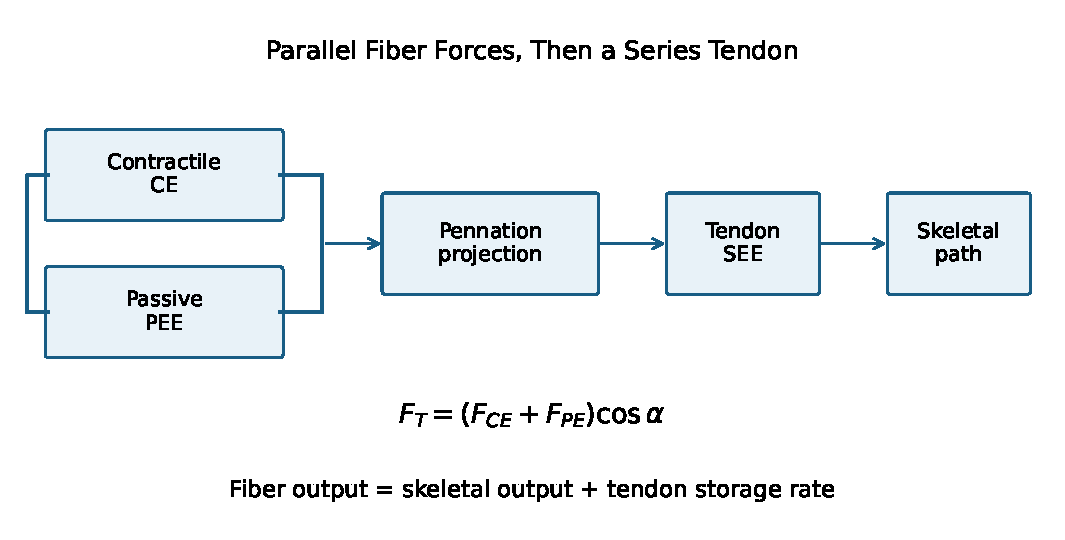
\includegraphics[width=\linewidth]{figures/muscle_force_network.pdf}
\caption{Force and Energy Connections in the Teaching Model. Active and Passive Fiber Forces Add Before Pennation Projection; the Tendon Is in Series.}
\label{fig:hill-muscle-model}
\end{figure}

The active and passive forces used here are
\begin{equation}
F_{\mathrm{CE}}=aF_0 f_L(\lambda)f_V(w),
\label{eq:ce-force}
\end{equation}
\begin{equation}
F_{\mathrm{PE}}=F_0f_P(\lambda).
\label{eq:pee-force}
\end{equation}
Let tendon slack length be $L_s$ and strain be $\epsilon=(\ell^T-L_s)/L_s$. Define a tendon force law independently of the passive fiber curve:
\begin{equation}
F_T(\epsilon)=
\begin{cases}
0,&\epsilon\leq0,\\
F_{\mathrm{ref}}\dfrac{e^{k_T\epsilon/\epsilon_{\mathrm{ref}}}-1}{e^{k_T}-1},&\epsilon>0.
\end{cases}
\label{eq:see-force}
\end{equation}
Here $F_{\mathrm{ref}}$ is the tendon force at positive reference strain $\epsilon_{\mathrm{ref}}$, and $k_T$ is dimensionless. Tendon tangent stiffness is $dF_T/d\ell^T$, measured in $\mathrm{N/m}$; it is not $k_T$. On the loaded branch,
\[
\frac{dF_T}{d\ell^T}
=\frac{F_{\mathrm{ref}}k_T e^{k_T\epsilon/\epsilon_{\mathrm{ref}}}}
{L_s\epsilon_{\mathrm{ref}}(e^{k_T}-1)}.
\]
The idealization stores energy without hysteretic loss. Actual loading and unloading may require a richer constitutive model. As with the passive fiber curve, the slack transition is continuous but not differentiable here.

\subsection{Geometry Connects Fiber, Tendon and Joint Motion}

Write the total path length as $\ell^{MT}=\ell^T+\ell^M\cos\alpha$. To differentiate it, specify how pennation changes. In a fixed-height model, $h=\ell^M\sin\alpha$ is constant, so
\[
\ell^M\cos\alpha=\sqrt{(\ell^M)^2-h^2}.
\]
Differentiating gives
\[
\dot\ell^M=\cos\alpha\,(\dot\ell^{MT}-\dot\ell^T).
\]
The relation applies for $\ell^M>h$; approaching $90^\circ$ pennation is a degenerate geometry, not an ordinary operating state. Assuming constant angle instead would give a different velocity relation. Combining fixed-height kinematics with the force projection gives the power identity
\[
F_T\dot\ell^{MT}=F_M\dot\ell^M+F_T\dot\ell^T.
\]
For example, $\ell^M=0.10\,\mathrm{m}$ and $h=0.06\,\mathrm{m}$ give $\cos\alpha=0.8$. If the path shortens at $0.10\,\mathrm{m/s}$ while the tendon lengthens at $0.02\,\mathrm{m/s}$, the fiber shortens at $0.096\,\mathrm{m/s}$. With $F_M=100\,\mathrm{N}$ and $F_T=80\,\mathrm{N}$, the identity is $-8=-9.6+1.6\,\mathrm{W}$. Of the fiber's mechanical output, $1.6\,\mathrm{W}$ is going into tendon storage at that instant. Tendon compliance therefore changes the fiber's velocity and its force capacity as well as storing energy.

For independent joint coordinates $q$ with $v=\dot q$, virtual work connects path length to moment arms:
\[
r_{ji}(q)=-\frac{\partial\ell_i^{MT}}{\partial q_j},
\qquad \dot{\boldsymbol\ell}^{MT}=-r^T v,
\qquad \boldsymbol\tau_M=r\boldsymbol F_T.
\]
For angular coordinates, entries of $r$ have units of meters per radian, conventionally written meters. Generalized coordinates that include translations require the corresponding force units; a model using $\dot q=N(q)v$ must include that mapping. The convention above ensures
\[
\boldsymbol\tau_M^T v=-\boldsymbol F_T^T\dot{\boldsymbol\ell}^{MT}.
\]
Shortening under positive tension can deliver positive power to the skeleton. Tendon lengthening can instead absorb part of that work. These equations also reveal multi-joint coupling: a muscle crossing two joints can generate moments at both, and motions at the two joints can reinforce or cancel its path-length change.

Take the local path in meters, with angles in radians:
\[
\ell^{MT}=0.30-0.02q_1+0.01q_2.
\]
 Its moment arms are $(0.02,-0.01)\,\mathrm{m}$. At $v=(10,20)\,\mathrm{rad/s}$, the path velocity is zero despite motion at both joints. At $v=(10,0)$, it is $-0.20\,\mathrm{m/s}$. Rigid translation of the entire arm and muscle together contributes no intrinsic path-length change. These examples explain why a clubhead or hand speed is insufficient to calculate muscle force.

\begin{principle}{Energy Storage and Release in the Tendon}{principle:see-energy}
Stored energy is the integral of force over extension, not force over dimensionless strain alone:
\[
U_T(\epsilon)=L_s\int_0^\epsilon F_T(s)\,ds.
\]
For positive strain in our law,
\[
U_T=\frac{F_{\mathrm{ref}}L_s}{e^{k_T}-1}
\left[\frac{\epsilon_{\mathrm{ref}}}{k_T}
\left(e^{k_T\epsilon/\epsilon_{\mathrm{ref}}}-1\right)-\epsilon\right].
\]
Set $F_{\mathrm{ref}}=100\,\mathrm{N}$, $L_s=0.20\,\mathrm{m}$, $\epsilon_{\mathrm{ref}}=0.04$ and $k_T=3$. At the reference strain, extension is $0.008\,\mathrm{m}$ and stored energy is $0.22475\,\mathrm{J}$. Differentiating energy with respect to extension recovers force. This provides a direct check on the units and expression.
\end{principle}

For the lossless model, $\dot U_T=F_T\dot\ell^T$. Substituting into the power identity shows that tendon recoil can add to instantaneous power delivered to the skeleton while its stored energy falls. It does not create energy. A shaft also stores and returns elastic energy, but its distributed bending and torsion, boundary conditions and contact with the golfer are different from a tendon model. Neither elastic mechanism by itself proves a universal benefit from a particular wrist action or shaft flexibility. The timing and direction of energy delivery must serve the impact task.

Force equilibrium must hold throughout this calculation. Arbitrarily prescribing activation, fiber length, fiber velocity and tendon extension independently can violate it. Some equilibrium formulations solve an inverse force-velocity relation for fiber velocity; zero activation or extreme geometry can make that inversion singular or impossible. A simulator must document how it handles such states. A numerical minimum activation is a modeling choice, not evidence that a person cannot cease neural excitation. \citep{millard2013flexing}

\section{How Muscle Biology Maps to Control Theory}

Mechanical position and velocity alone do not generally specify the future of an activated, compliant muscle system. Two otherwise identical poses can have different activation and tendon loading because of their histories. A useful state for this teaching model is
\begin{equation}
x=(q,v,\boldsymbol a,\boldsymbol\ell^M),\qquad \dot x=f(x)+G(x)\boldsymbol u.
\label{eq:control-affine-remit}
\end{equation}
For $n$ independent mechanical coordinates and $m$ modeled muscle compartments,
\begin{equation}
\boldsymbol u\in[0,1]^m,
\label{eq:neural-command}
\end{equation}
\begin{equation}
\boldsymbol a\in[0,1]^m,
\label{eq:activation-vector}
\end{equation}
\begin{equation}
\boldsymbol F_T\in\mathbb R_{\geq0}^m,
\label{eq:force-vector}
\end{equation}
\begin{equation}
\boldsymbol\tau_M=r(q)\boldsymbol F_T\in\mathbb R^n.
\label{eq:torque-from-muscles}
\end{equation}
There is no fixed universal number of actuators per joint. One anatomical muscle may be split into compartments, and one compartment may span multiple joints. Excitations are bounded; tendon forces are tensile; admissible forces also depend on equilibrium and the current state. They are not arbitrary unconstrained control vectors.

Away from an impact event, a specified unconstrained mechanical model may take the form
\[
\dot v=A(x)=M(q)^{-1}\{r(q)\boldsymbol F_T(x)
+\boldsymbol b_{\mathrm{ext}}(x)-\boldsymbol c(q,v)-\boldsymbol g(q)\}.
\]
$M$ is the mass matrix, $\boldsymbol c$ the velocity-dependent inertial terms, $\boldsymbol g$ the gravitational terms and $\boldsymbol b_{\mathrm{ext}}$ specified external generalized forces. Contact constraints, unknown reaction forces or a flexible shaft require the corresponding additional equations. A collision may require an impulse or compliant-contact treatment; the smooth equation should not silently be applied across it.

Suppose a well-defined muscle equilibrium solution gives $\dot{\boldsymbol\ell}^M=\Phi(x)$, and activation constants form the diagonal matrix $T_a$. Then the actual augmented control-affine expression is
\begin{equation}
f(x)=\begin{bmatrix}v\\A(x)\\-T_a^{-1}\boldsymbol a\\\Phi(x)\end{bmatrix},
\qquad
G(x)=\begin{bmatrix}0_{n\times m}\\0_{n\times m}\\T_a^{-1}\\0_{m\times m}\end{bmatrix}.
\label{eq:control-affine-full}
\end{equation}
Excitation enters the activation derivative, not the mechanical acceleration directly. Its mechanical effect develops as the state evolves. The component units differ appropriately: position rate, acceleration, activation rate and fiber-length rate. Equating $G\boldsymbol u$, a state-rate vector, with a scalar joint torque would be dimensionally incorrect. This expression also depends on a fixed $T_a$ and an admissible $\Phi$ independent of instantaneous excitation. If the activation time constant switches with $u$ and $a$, global affinity in $u$ no longer follows from this display.

\begin{laymansbox}{Why Effective Control Depends on State and Time}{context:gain-decreases}
At fixed length and velocity, the active force's sensitivity to activation is proportional to $F_0 f_L f_V$. During shortening, that sensitivity can decline as local fiber speed rises. The resulting joint effect also depends on moment arms, the mass matrix, tendon dynamics and other joints. A new excitation change has no instantaneous jump effect on activation in this model. A previously prepared activation can still produce force, and a loaded tendon can still recoil, even if the current excitation is zero.
\end{laymansbox}

\begin{example}{Numerical Estimate: Finite-Horizon Joint Response}{control-gain}
Consider a deliberately simple joint with constant inertia $I=0.10\,\mathrm{kg\,m^2}$. An added actuator torque is $\tau_{\max}a(t)$, with $\tau_{\max}=2\,\mathrm{N\,m}$, $a_0=0$, $u=1$ and $\tau_a=0.025\,\mathrm{s}$. Holding all other torques equal between two trajectories, the changes after a remaining response duration $T$ are
\[
\Delta v=\frac{\tau_{\max}}{I}\left[T-\tau_a(1-e^{-T/\tau_a})\right],
\]
\[
\Delta q=\frac{\tau_{\max}}{I}
\left[\frac{T^2}{2}-\tau_aT+\tau_a^2(1-e^{-T/\tau_a})\right].
\]
At $T=0.050\,\mathrm{s}$, $\Delta q=0.0108083\,\mathrm{rad}$, or about $0.6193^\circ$. This is a finite-horizon response from explicit initial conditions, not a predicted golf correction. A specified pure delay is removed from the available interval before using $T$; if no response time remains, this command produces no pre-impact effect in this model. Existing activation, elastic loading and configuration-dependent dynamics require a different calculation.
\end{example}

\subsection{Drift, Cancellation and Reachability}

In the mechanical equation, a conventionally defined non-muscle generalized term is
\begin{equation}
\boldsymbol b_{\mathrm{mech}}=
\boldsymbol b_{\mathrm{ext}}-\boldsymbol c-\boldsymbol g.
\label{eq:drift-torque}
\end{equation}
Its definition must say which external forces and passive effects it includes. In the augmented state equation, the zero-input drift also includes ongoing activation and stored elastic state. Therefore zero excitation is not equivalent to zero muscle force or purely gravitational motion. And $I\ddot q$ inferred from observed acceleration is the total required inertial balance in a scalar model, not an independently measured free-drift torque.

Suppose a scalar mechanical term is $-80\,\mathrm{N\,m}$ and an added control moment can range from $-4$ to $4\,\mathrm{N\,m}$. With positive constant inertia, all available accelerations have the same sign. Nevertheless, their magnitudes differ and their velocity and position trajectories separate over time. Inability to cancel the current acceleration is not inability to influence the eventual state. Conversely, a favorable instantaneous torque ratio does not guarantee that the required impact state is reachable within the remaining time and actuator bounds.

For the golf question, compare admissible policies over a stated horizon with the same starting mechanical, activation and elastic states. Measure their effects on clubface orientation, impact location and velocity, while checking other joint loads and contact conditions. A linearized sensitivity of these outputs to excitation can be informative, but it must follow the trajectory and its state transitions. A ratio evaluated at one joint at one instant cannot establish nonlinear controllability, global optimality or injury risk.

\section{Muscle Force in the Golf Swing: What Numbers Establish}

\begin{principle}{Peak Torques at Major Golf Joints}{principle:peak-torques}
Three kinds of number answer different questions. A maximum isometric test estimates capacity in a specified posture and protocol. Inverse dynamics estimates the net generalized moment consistent with measured motion and external forces under a chosen model. A force plate measures an external ground wrench, which must be transformed and combined with segment dynamics before assigning internal joint moments. Comparing them requires matched coordinate conventions, units, populations and loading conditions. None is automatically an individual muscle-force measurement.
\end{principle}

For two antagonists with moment arms $(0.02,-0.02)\,\mathrm{m}$, tendon forces $(100,0)\,\mathrm{N}$ and $(200,100)\,\mathrm{N}$ both produce $2\,\mathrm{N\,m}$ net torque. Their summed tensions are $100$ and $300\,\mathrm{N}$. Thus a low net torque can coexist with substantial opposing forces. Joint compression, stiffness and metabolic cost require their own geometry and constitutive models; they cannot be recovered from that torque equality. An optimization algorithm may select one force allocation, but its objective and constraints provide information that inverse dynamics alone does not contain.

EMG is useful for investigating electrical activity, but it is not a calibrated force meter. Roberts and Gabaldón's direct force, fascicle and EMG measurements in turkey hindlimb muscles illustrate that their relationships can vary across movement conditions. That finding supports distinguishing the signals; it does not calibrate human forearm force during golf. \citep{RobertsGabaldon2008EMG} A golf study needs its own measurement model, normalization choices and uncertainty analysis.

\begin{principle}{Muscle Capacity and Mechanical Demand}{muscle-demand-phases}
Earlier actions can change later geometry, velocity, activation and tendon loading. Later actions can change the trajectory within their remaining response time and bounds. A sequence that reduces one muscle's shortening speed may improve its active-force capacity while increasing demand elsewhere. A motion that increases elastic storage may also change joint loading or mistime recoil. These are coupled tradeoffs, so no universal early-effort/late-coast rule follows from a single force curve.
\end{principle}

To evaluate a proposed sequence, first state the desired impact outputs and acceptable variability. Next estimate the mechanical and muscle states consistently, identifying parameters inferred rather than measured. Finally compare alternatives with the same task and initial conditions, including sensitivity to moment arms, slack lengths, activation constants and measurement error. Agreement with a net torque curve is useful but insufficient validation of every internal force. A stronger claim should survive independent observations relevant to the proposed mechanism.

\section{Implications for Swing Mechanics and Training}

\begin{principle}{Interpreting the Cue to Accelerate Through Impact}{accelerate-to-impact}
A coaching cue is not a direct report of muscle force or clubhead acceleration. Continuing effort can coexist with a declining shortening-force multiplier, and clubhead speed can increase through coupled motion while a particular muscle does little positive work. Evaluate the cue by its repeatable effect on the intended impact outcomes and by an appropriate mechanical explanation. The equations here neither require every muscle to accelerate the club until contact nor prove that all late effort is harmful.
\end{principle}

Training can alter capacity, coordination and how a player prepares the state entering the downswing. These mechanisms need different tests. Greater isometric strength does not by itself establish greater available force at the relevant fiber lengths and velocities; a successful practice swing does not establish improved retention or transfer. A useful investigation links the proposed change to a measured outcome and checks whether the inferred mechanism is consistent with the full movement. This keeps practical instruction informative while leaving uncertainty visible.

\begin{principle}{Key Takeaways: Muscle Force Generation}{principle:muscle-takeaways}
Trace the chain from excitation to activation, fiber force, tendon force, joint moments and task outputs. Keep local fiber velocity distinct from club speed. Preserve force equilibrium and virtual work when joining geometry to mechanics. Account for the energy and activation already present at the start of a comparison. Interpret net moments, EMG and capacity measurements according to what each measures. Judge control over the remaining trajectory, and test proposed golf sequences against alternatives rather than declaring one optimal from an instantaneous ratio.
\end{principle}

\subsection{Looking Ahead}
The muscle-to-joint and movement-control chapters use these distinctions at larger scales. Multi-joint geometry determines how muscle forces influence motion; activation and tendon memory determine what the same current command can do; learning determines how a player prepares and adjusts those states. Together they make the golf swing a question about coordinated trajectories and impact outcomes, not an isolated contest between one muscle and one inertial number.

\begin{exercises}{Chapter Exercises}{ex:muscle-chapter}
All numerical parameters below belong to the teaching model, not a golfer dataset.
\begin{enumerate}
\item For the Gaussian with $\gamma=0.5$, calculate $f_L$ at $\lambda=0.8$, $1.2$ and $1.5$. Does it have any finite zero? At $\lambda=1.2$, calculate total force divided by $F_0$ for $a=0.7$, $w=0$ and the stated passive curve.
\item Use $r=0.02\,\mathrm{m}$, $\dot q=8.75\,\mathrm{rad/s}$, $\ell^M_{\mathrm{opt}}=0.10\,\mathrm{m}$ and $\nu=10\,\mathrm{s^{-1}}$. Assume a rigid tendon, zero pennation and shortening in the positive joint direction. Calculate $w$, $f_V$ and torque for $F_0=100\,\mathrm{N}$ at optimal length and full activation.
\item For $\tau_a=25\,\mathrm{ms}$, $a_0=0$ and $u=1$, find the $50\%$ and $95\%$ activation times. Compare the latter with forward Euler using $5\,\mathrm{ms}$ steps. Explain why neither is a pure neural delay.
\item A path shortens by $0.02\,\mathrm{m}$ per radian of $q_1$ and lengthens by $0.01\,\mathrm{m}$ per radian of $q_2$. Find both moment arms and path velocity at $v=(10,20)\,\mathrm{rad/s}$. With $F_T=100\,\mathrm{N}$, calculate the two joint powers and their sum. Assume no other path dependence.
\item Derive the finite-horizon formulas by integrating $\Delta\ddot q=K a(t)$, where $K=\tau_{\max}/I$ and $a(t)=1-e^{-t/\tau_a}$. Use zero initial position and velocity differences. Evaluate $\Delta q$ after $50\,\mathrm{ms}$ using the chapter's parameters. Explain why a small instantaneous torque ratio does not set this result to zero.
\item Use $F_{\mathrm{ref}}=100\,\mathrm{N}$, $L_s=0.20\,\mathrm{m}$, $\epsilon_{\mathrm{ref}}=0.04$ and $k_T=3$. Find force, extension and energy at the reference strain. Verify $dU_T/d\ell^T=F_T$, and identify the dimensional error in integrating force over strain without $L_s$.
\item Design a comparison of two proposed swing sequences. State the common initial conditions, task outcomes, muscle-state estimates and uncertain parameters. Identify one observation that would distinguish a change in muscle timing from a change in geometry or tendon loading.
\end{enumerate}
\end{exercises}

\subsection{Worked Answers}
\begin{enumerate}
\item The multipliers are $0.8521$, $0.8521$ and $0.3679$; none is zero. Total normalized force is approximately $0.7188$, including $0.12227$ passive force. The Gaussian remains positive at every finite argument.
\item $V_{\max}=1\,\mathrm{m/s}$, $w=0.175$, $f_V\approx0.5739$, force $57.39\,\mathrm{N}$ and moment $1.148\,\mathrm{N\,m}$. A linear calculation would give a different answer because it is a different law.
\item $t_{50}=17.33\,\mathrm{ms}$ and $t_{95}=74.89\,\mathrm{ms}$. Euler first exceeds $95\%$ at step 14, $70\,\mathrm{ms}$. The continuous response begins immediately in this model; the time constant controls its rate of approach.
\item The moment arms are $(0.02,-0.01)\,\mathrm{m}$ and path velocity is zero. Torques $(2,-1)\,\mathrm{N\,m}$ produce powers $(20,-20)\,\mathrm{W}$, summing to zero. Opposite joint powers can coexist with no net muscle-tendon shortening power.
\item Integrate once for velocity and again for position, retaining both integration constants fixed by the initial conditions. The position difference is $0.0108083\,\mathrm{rad}$, about $0.6193^\circ$. A torque too small to cancel another term can still accumulate a trajectory difference.
\item Force is $100\,\mathrm{N}$, extension $0.008\,\mathrm{m}$ and energy $0.22475\,\mathrm{J}$. Since $d\epsilon/d\ell^T=1/L_s$, differentiating the energy cancels the slack-length factor and returns force. Without that factor, the strain integral has units of newtons rather than joules.
\item One defensible design matches the task and starting body, club, activation and elastic states, then compares feasible excitation histories. Record impact orientation, location and velocity as well as relevant loads. Use synchronized motion and electrical signals, with a validated force/geometry model and, where feasible, independent fascicle or tendon measurements. Test parameter sensitivity and predictions not used for fitting. A timing claim should explain observations that an alternative geometry or elastic-state change does not explain equally well; otherwise the mechanism remains underdetermined.
\end{enumerate}
\clearpage
\flushbottom{}
